\documentclass[12pt,openany]{report}
\usepackage{alltt,epsfig,html,latexsym,longtable,makeidx,moreverb}

\setlength\topmargin{-0.5in}
\setlength\textheight{8.5in}
\setlength\textwidth{7.0in}
\setlength\oddsidemargin{-0.3in}
\setlength\evensidemargin{-0.3in}
\hyphenation{}
\title{{\mlton} Hacker Guide}
\author{Stephen Weeks}
\date{\today}
\newcommand{\absolutelink}[1]{\link{\makeurl{#1}}}
\newcommand{\addr}{mlton.org}
\newcommand{\chaplab}[1]{\label{chapter:#1}}
\newcommand{\chapref}[1]{Chapter~\ref{chapter:#1}}
\newcommand{\chap}[2]{\chapter{#1}{\chaplab{#2}}}
\newcommand{\code}[1]{\htmladdnormallink{{\tt #1}}{../../#1}}
\newcommand{\deflab}[1]{\label{definition:#1}}
\newcommand{\defref}[1]{Definition~\ref{definition:#1}}
\newcommand{\figBegin}{\begin{figure}\begin{boxit}}
\newcommand{\figEnd}[2]{\caption{#1}\figlab{#2}\end{boxit}\end{figure}}
\newcommand{\figlab}[1]{\label{figure:#1}}
\newcommand{\figref}[1]{Figure~\ref{figure:#1}}
\newcommand{\lemlab}[1]{\label{lemma:#1}}
\newcommand{\lemref}[1]{Lemma~\ref{lemma:#1}}
\newcommand{\link}[1]{\htmladdnormallink{{\tt #1}}{#1}}
\newcommand{\mailto}[1]{\htmladdnormallink{{\tt #1}}{mailto:#1}}
\newcommand{\makeurl}[1]{http://www.\addr/MLton/#1}
\newcommand{\mltonmail}{\mailto{MLton@\addr}}
\newcommand{\mlton}{MLton}
\newcommand{\mosml}{Moscow ML}
\newcommand{\place}[1]{\item[\tt #1]\hspace{1in}\\}
\newcommand{\seclab}[1]{\label{section:#1}}
\newcommand{\secref}[1]{Section~\ref{section:#1}}
\newcommand{\smlnj}{SML/NJ}
\newcommand{\subsecc}[2]{\subsubsection{#1}\seclab{#2}}
\newcommand{\subsec}[2]{\subsection{#1}\seclab{#2}}
\newcommand{\subsubsec}[2]{\subsubsection{#1}\label{section:#2}}
\newcommand{\tabBegin}{\begin{table}}
\newcommand{\tablab}[1]{\label{table:#1}}
\newcommand{\tabref}[1]{Table~\ref{table:#1}}
\newcommand{\thmlab}[1]{\label{theorem:#1}}
\newcommand{\thmref}[1]{Theorem~\ref{theorem:#1}}
\newcommand{\userguide}{{\mlton} User Guide}
\newcommand{\version}{VERSION}
\renewcommand{\sec}[2]{\section{#1}\seclab{#2}}
\newenvironment{boxit}{\vbox\bgroup\hrule\hbox\bgroup\vrule\kern3pt\vbox\bgroup\kern3pt\advance\hsize by -6.8pt\relax}{\par\kern3pt\egroup\kern3pt\vrule\egroup\hrule\egroup}

\makeindex

\begin{document}

\maketitle
This document describes how to hack {\mlton}, a
whole-program optimizing compiler for the
\htmladdnormallink{Standard ML}
                  {http://cm.bell-labs.com/cm/cs/what/smlnj/sml.html}
programming language.
The {\mlton} homepage is \absolutelink{}.
The document contains an overview of the source tree, a description of the
programming style used in {\mlton}, and delves into the bowels of the compiler
and associated tools.

This document is very incomplete.  

\tableofcontents
\chap{The sources}{sources}

This section is an overview of the sources to the compiler and all of the
associated tools.  Here is a brief description of each element of the root
source directory.  Throughout the rest of this document, we will use pathnames
that are relative to the source directory.

\begin{description}

\place{basis-library}
The basis library implementation.
\place{benchmark}
Code and tests used for benchmarking {\mlton}, {\smlnj}, and {\mosml}.
\place{bin}
Scripts for type checking the basis library, making rpms, running {\mlton}, and
running regression tests.
\place{doc}
Sources for the user guide, hacker guide, web site, announcements, README.
\place{include}
Include files needed for compiling C files generated by {\mlton}.
\place{lib}
SML library code, which is used in {\tt mlton}, {\tt mlprof}, and {\tt
benchmark}.  There are also many generally useful libraries.
\place{Makefile}
To make everything.  This is only used when building rpms.
\place{man}
Manual pages for {\tt mlton} and {\tt mlprof}.
\place{mllex}
Lexer generator, taken and slightly modified from {\smlnj}.
\place{mlprof}
Profiler.
\place{mlton}
Compiler.
\place{mlyacc}
Parser generator, taken and slightly modified from {\smlnj}.
\place{regression}
Regression tests, about 150 SML files that are used to test the compiler.
\place{runtime}
Runtime system, which includes the garbage collector and C libraries used in
the basis (including the GMP used for {\tt IntInf}).

\end{description}

\chap{The basis library}{basis-library}

The basis library is implemented with about 12,000 lines of SML code.  There is
roughly one file for each signature and structure that the library specification
defines.  The files are grouped in directories in the same way that the
corresponding modules are grouped in the basis library documentation.  Here is
an overview of the {\tt basis-library} directory.

\begin{description}
\place{arrays-and-vectors general integer io list posix real system text}
SML code for basis library modules.

\place{basis.sml}
Automatically constructed by {\tt bin/check-basis}.  Used to type check the
basis libary under {\smlnj}.

\place{bind-basis}
A list of the files (in order) that define what is exported by the basis
library.

\place{build-basis}
A list of the files (in order) used to construct the basis library.

\place{Makefile}
Only has a target to clean the directory.

\place{misc}
SML code that didn't fit anywhere else.  In particular, the {\tt Primitive}
structure.

\place{mlton}
The {\tt MLton} structure, which is not part of the standard basis library.
For more details on what {\tt MLton} provides, see the {\userguide}.

\place{sml-nj}
The {\tt SMLofNJ} and {\tt Unsafe} structures, which are not part of the
standard basis library.

\place{top-level}
Files describing the overloads, infixes, modules, types, and values that the
basis library makes available to user programs.
\end{description}

\subsec{How {\mlton} builds the basis environment}{build-basis-env}
The {\tt forceBasisLibrary} function in \code{\tt mlton/main/compile.sml} builds
the basis environment that is used to compile user programs.  Conceptually, the
basis environment is constructed in two steps.  First, all of the files in {\tt
build-basis} are concatenated together and evaluated to produce an environment
$E$.  Then, all of the files in {\tt bind-basis} are concatenated and evaluated
in environment $E$ to produce a new environment $E'$, which is the top-level
environment.  Another way to view it is that every user program is prefixed by
the following.
\begin{verbatim}
local
  <concatenate files in build-basis>
in
  <concatenate files in bind-basis>
end
\end{verbatim}
This view is not strictly accurate because some of the files are not SML (they
use the {\tt \_prim}, {\tt \_ffi}, and {\tt \_overload} syntaxes) and because SML
does not allow local functor or signature declarations.  Here is a description
of the basis files that are not SML.
\begin{description}
\place{misc/primitive.sml}
Defines the {\tt Primitive} structure, which binds (via the {\tt \_prim}
syntax) all of the primitives provided by the compiler that the basis library
uses.
\place{mlton/syslog.sml}
Defines constants and FFI routines used to implement {\tt MLton.Syslog}.
\place{posix/primitive.sml}
Defines the {\tt PosixPrimitive} structrue, which binds the constants and FFI
routines used to implement the {\tt Posix} structure.
\place{top-level/overloads.sml}
Defines the overloaded variables available at the top-level the {\tt \_overload}
syntax: {\tt \_overload $x$: $ty$ as $y_0$ and $y_1$ and ...}
\end{description}

\subsection{Modifying the basis library}

If you modify the basis library, you should first check that your modifications
are type correct using the {\tt bin/check-basis} script.  Since this {\mlton}
does not have a proper typechecker, this script uses {\smlnj}.  First, it
concatenates the files as described in \secref{build-basis-env} into one file,
{\tt basis.sml}.  It also replaces the nonstandard syntax ({\tt \_prim}, etc.) 
and declares the toplevel types to match {\mlton}'s (necessary since {\smlnj}
uses 31 bits while {\mlton} uses 32).  It then feeds {\tt basis.sml} to
{\smlnj}.  If there are no type errors, a message like the following will
appear.
\begin{verbatim}
stdIn:12213.1-12213.14 Error: operator is not a function [tycon mismatch]
  operator: unit
  in expression:
    () ()
\end{verbatim}
This error message is intentionally introduced by {\tt check-basis} at the end
of {\tt basis.sml} to make it clear that {\smlnj} reached the end of {\tt
basis.sml} and has hence type checked the entire basis.

Once you have a basis library that type checks, you need to create a new version
of {\mlton} that uses this library.  {\mlton} preprocess the basis library to
create a {\tt world.mlton} file that contains the basis environment.  The {\tt
world.mlton} file is stored in the {\tt lib} directory and is loaded by {\tt
mlton} when compiling a user program (see the {\tt bin/mlton} script).  To build
a new {\tt world.mlton}, run {\tt make world} from within the sources directory.

\subsection{The {\tt misc} directory}

\begin{description}

\place{cleaner.sig}
Functions for register ``cleaning'' functions to be run at certain times, in
particular at program exit.  The {\tt TextIO} module uses these cleaners to
ensure that IO buffers are flushed upon exit.

\place{suffix.sml}
Code that is (conceptually) concatenated on to the end of every user program.
It just calls {\tt OS.Process.exit}.  The {\tt forceBasisLibrary} function
ensures that {\tt suffix.sml} is elaborated in an environment where the basis
library {\tt OS} structure is available.

\place{top-level-handler.sml}
This defines the top level exception handler that is installed (via a special
compiler primitive) in the basis library, before any user code is run.

\end{description}

\subsection{Dead-code elimination}

In order to compile small programs rapidly and to cut down on executable size,
{\tt mlton} runs a pass of dead-code elimination ({\tt
mlton/core-ml/dead-code.sig}) to eliminate as much of the basis library as
possible.  The dead-code elimination algorithm used is not safe in general, and
only works because the basis library implementation has special properties:
\begin{itemize}
\item it terminates
\item it performs no I/O
\item it doesn't side-effect top-level variables
\end{itemize}
The dead code elimination simply includes the minimal set of
declarations from the basis so that their are no free variables in the
user program (or basis).  Hence, if you do something like the
following in the basis, it will break.
\begin{verbatim}
val r = ref 13
val _ = r := 14
\end{verbatim}
The dead code elimination will remove the {\tt val \_ = ...} binding.

\chap{The runtime}{runtime}
\section{Notes}

There are multiple, possibly orthogonal issues.  Limit checks and garbage
collections are a little overloaded in their roles, because they also
support preemptive thread switching and interrupt handling.  Forcing
frontier to be 0 and hitting a limit check (even a zero byte limit check)
will invoke the GC, which will switch to the pending thread.

Recall that a limit check with bytes = 0 really means a check for LIMIT\_SLOP
bytes (currently LIMIT\_SLOP = 512).

\section{Bootstrap}

\figBegin
\centerline{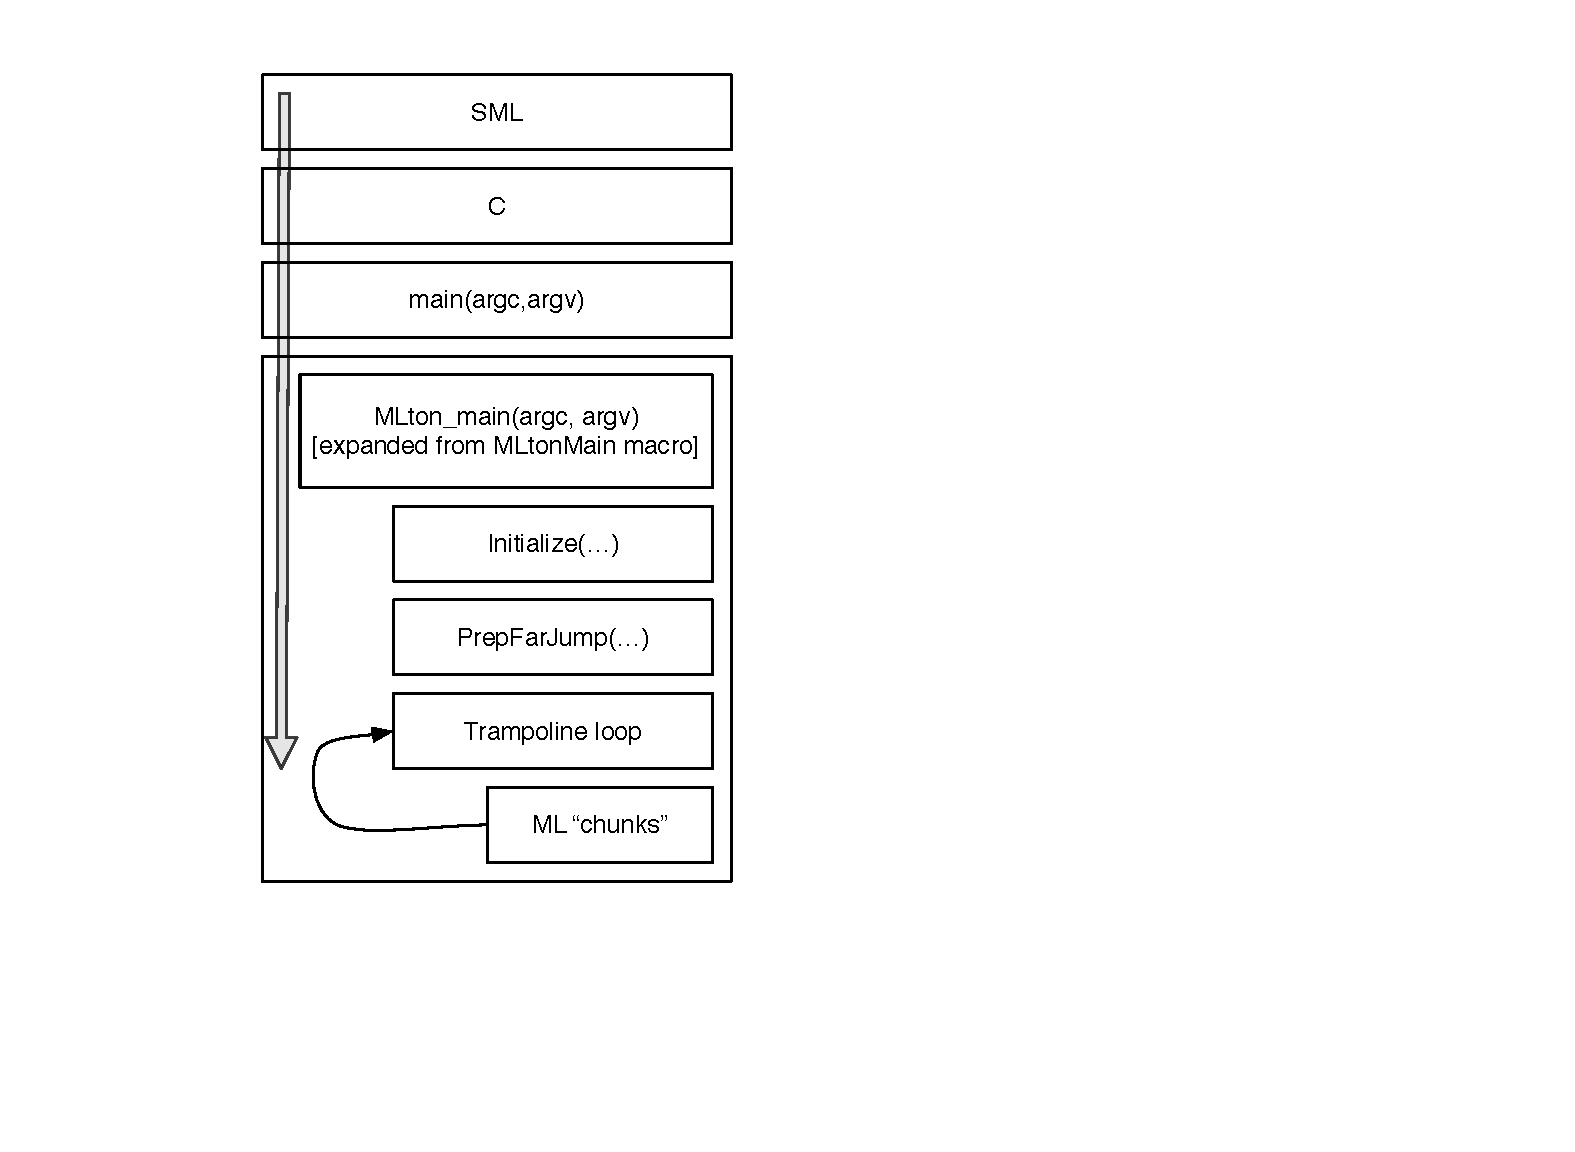
\epsfig{file=runtime-bootstrap-overview.pdf,width=2.0in}}
\figEnd{Runtime overview}{rtoverview}
       
When you compile your SML code, it is translated to machine code using one of several backends. For an in-depth description of how SML is compiled and optimized refer to~\cite{leibig:mlton-llvm-backend}. We will look at the C translation of a trivial SML program starting at the backend once all optimization phases have completed. The trivial SML program is a single statement: \texttt{val a = 2}

When reading this section of the guide, it will be useful to save the above statement as "test.sml" and then compile that using "mlton -keep g test.sml" so that you can refer to the intermediate files "test.0.c" "test.1.c" and "test.2.c"

Refer to Figure~\ref{figure:rtoverview} for an overview of how the compiler emits C code given SML code, and how control flows through the bootstrap process of the emitted code.

 
The emitted C code bootstrap at the bottom of "test.0.c" looks like this:

\begin{minipage}{\linewidth}
\lstset{language=C}\begin{lstlisting}
MLtonMain (8, 0x7CB29B69, 136, TRUE, PROFILE_NONE, FALSE, 0, 218)
int main (int argc, char* argv[]) {
    return (MLton_main (argc, argv));
}
\end{lstlisting}
\end{minipage}

\noindent and contains a \texttt{main} routine that calls \texttt{MLton\_main} which is created when the \texttt{MLtonMain} macro is expanded. 
\texttt{MLtonMain} is defined in \texttt{include/c-main.h} as a macro:

\begin{minipage}{\linewidth}
\lstset{language=C}\begin{lstlisting}
#define MLtonMain(al, mg, mfs, mmc, pk, ps, mc, ml)	
\end{lstlisting}
\end{minipage}

and ultimately calls the routine \texttt{MLton\_main (int argc, char* argv[])} which 

The parameters to the \texttt{MLtonMain} macro are:

\setlist[description]{leftmargin=!,labelindent=\parindent,labelwidth=1.5cm}

\begin{description}
\item[al] alignment width (\texttt{-align})
\item[mg] a magic random number used for saving/restoring the world. This number is generated at compile time by \texttt{mlton/codegen/c-codegen/c-codegen.fun} and allows the application to save and restore its state (\htmladdnormallink{MLtonWorld}{http://mlton.org/MLtonWorld})
\item[mfs] the maximum frame size
\item[mmc] whether or not the mutator marks cards. This is an optimization strategy used by the generational GC.
\item[pk] the kind of profiling to perform (compile time option)
\item[ps] whether stack profiling is enabled (\texttt{-profile-stack})
\item[mc] the number of the first chunk to jump to
\item[ml] the function number in the chunk to jump to
\end{description}

The first six of these parameters are passed to \texttt{Initialize} (defined in \texttt{include/common-main.h}) while the final two (mc and ml) are passed to \texttt{PrepFarJump} (defined in \texttt{include/c-common.h}). 
\texttt{Initialize} sets variables in the \texttt{gcState} structure and then calls \texttt{MLton\_init(argc, argv, \&gcState)}.



\texttt{MLton\_init} (\texttt{runtime/platform.c}) initializes the posix environment, the GC and processes the runtime command line arguments.  Once \texttt{Initialize} completes, \texttt{MLton\_main} continues and calls \texttt{PrepFarJump} to prepare to jump to the first chunk of the SML program. Alternatively, it will restore the saved world and restart from where the saved program left off. Finally, \texttt{MLton\_main} goes into an infinite loop, jumping from chunk to chunk as the SML program executes.

Jumping between chunks is known as trampolining and this is done to avoid mapping highly recursive SML functions directly to C functions as this would exhaust the C stack (see \S2.2.4 of~\cite{leibig:mlton-llvm-backend}). Trampolining involves selecting a chunk from the \texttt{cont} struct and then calling to that address (pointer). You will notice that, in our example above, \texttt{mc} is set to 0 and \texttt{ml} is set to 218. That means that \texttt{PrepFarJump} will select chunk 0 to execute and will set the next function within chunk zero to 218. 

So walking through this, \texttt{SetFarJump(0, 218)} will result in 

\begin{minipage}{\linewidth}
\lstset{language=C}\begin{lstlisting}
cont.nextChunk = (void *)Chunk0;
nextFun = 218;
\end{lstlisting}
\end{minipage}

The \texttt{Chunk0} symbol is declared in "test.0.c" via the \texttt{DeclareChunk (0)} line. This is a macro that expands to 

\begin{minipage}{\linewidth}
\lstset{language=C}\begin{lstlisting}
PRIVATE struct cont Chunk0(void);
\end{lstlisting}
\end{minipage}

The actual \texttt{Chunk0} routine is defined in "test.2.c" via the line \texttt{Chunk (0)} which is another macro (defined in \texttt{include/c-chunk.h} that expands to:

\begin{minipage}{\linewidth}
\lstset{language=C}\begin{lstlisting}
	
        DeclareChunk(0) {
                struct cont cont;
                Pointer frontier;
                uintptr_t l_nextFun = nextFun; // remember this is 218
                Pointer stackTop;
\end{lstlisting}
\end{minipage}

Where \texttt{DeclareChunk} is, you guessed it, a macro (defined in \texttt{include/c-common.h}) and so results in the above expanding to:


\begin{minipage}{\linewidth}
\lstset{language=C}\begin{lstlisting}
PRIVATE struct cont Chunk0(void) {
                struct cont cont;
                Pointer frontier;
                uintptr_t l_nextFun = nextFun; // remember this is 218
                Pointer stackTop;
\end{lstlisting}
\renewcommand{\lstlistingname}{Code}
\end{minipage}

And so we finally have our \texttt{Chunk0} routine which is what we set \texttt{chunk.nextChunk} to above if you recall.





Given the above, the trampoline section of \texttt{MLton\_main} (again, in \texttt{include/c-main.h}) will call


\begin{minipage}{\linewidth}
\lstset{language=C}\begin{lstlisting}
cont=(*(struct cont(*)(void))cont.nextChunk)(); 
\end{lstlisting}
\end{minipage}

We will see, as we fully expand \texttt{Chunk0} how it ultimately returns a \texttt{cont} structure to allow us to trampoline to the next chunk. Also, we will see how each chunk routine is a large \texttt{switch} statement indexed by nextFun and so, architecturally, MLton aggregates SML functions into large C-functions where each SML function is one of the cases in the switch statement. This is how MLton minimizes the growth of the C-stack.

Continuing on, we are now in the \texttt{Chunk0} routine which we see, from examining "test.2.c" continues past the \texttt{Chunk (0)} line as such:

\begin{minipage}{\linewidth}
\lstset{language=C}\begin{lstlisting}
Chunk (0)
        CPointer Q_0;
        CPointer Q_1;
        CPointer Q_2;
	.
	.
	.
ChunkSwitch (0)
case 5:
L_9:
        Push (-8);
	.
	.
	.
case 218:
        G(Word32, 0) = CPointer_lt (O(CPointer, GCState, 40), StackTop);
        BNZ (G(Word32, 0), L_8);
        G(Word64, 0) = CPointer_diff (O(CPointer, GCState, 1360), Frontier);
        G(Word32, 1) = WordU64_lt (G(Word64, 0), (Word64)(0x1090ull));
        BNZ (G(Word32, 1), L_8);
        goto L_2;
	.
	.
	.
EndChunk
\end{lstlisting}
\end{minipage}

Examining this routine, let's first look at the bottom \texttt{EndChunk} which is a macro (defined in \texttt{include/c-chunk.h}) and expands to:

\begin{minipage}{\linewidth}
\lstset{language=C}\begin{lstlisting}
                default:
                        /* interchunk return */
                        nextFun = l_nextFun;
                        cont.nextChunk = (void*)nextChunks[nextFun];
                        leaveChunk:
                                FlushFrontier();
                                FlushStackTop();
                                return cont;
                    } /* end switch (l_nextFun) */
                } /* end while (1) */
        } /* end chunk */	
\end{lstlisting}
\end{minipage}

This results in \texttt{nextFun} being set to the next function in the switch statement to execute and then it sets \texttt{cont.nextChunk} to the next chunk (if we need to switch between C functions) and finally it flushes some registers and returns. Note the label \texttt{leaveChunk} allows SML functions to jump out of the C function. The "end while (1)" refers to a while statement in the macro \texttt{ChunkSwitch} which we will now look at, before bringing this all together into a macro-less C fragment.

\chap{MLton}{mlton}

This chapter describes the compiler proper, which is found in the {\tt mlton}
directory.

\section{Sources}

\begin{description}

\place{ast}
Abstract syntax trees produced by the front end.

\place{atoms}
Common atomic pieces of syntax trees used throughout the compiler, like
constants, primitives, variables, and types.

\place{backend}
The backend translates from the {\tt Cps} IL to a machine independent IL called
{\tt Machine}.  It decides data representations, stack frame layouts, and creates
runtime system information like limit checks and bitmasks.

\place{call-main.sml}
A one-line file that is the last line of the compiler sources.  It calls the
main function.

\place{closure-convert}
The closure converter, which converts from {\tt Sxml}, the higher-order
simply-typed IL, to {\tt Cps}, the first-order simply-typed IL.

\place{cm}
Support for {\smlnj}-style compilation manager (CM) files.

\place{codegen}
Both the C and the native X86 code generator.

\place{control}
Compiler switches used throughout the rest of the compiler.

\place{core-ml}
The implicitly typed IL that results from defunctorization.  Contains a
pass of dead code elimination for eliminating basis library code.  Also contains
the pass that replaces constants defined by {\tt \_prim} with their values.

\place{elaborate}
The elaborator, which matches variable uses with bindings in the AST IL and
defunctorizes to produce a {\tt CoreML} program.  It does not do type checking
yet, but will someday. 

\place{front-end}
The lexer and parser, which turn files into ASTs.

\place{main}
The two main structures in the compiler, one ({\tt Main}) for handling all the
command line switches and one ({\tt Compile}) which is a high-level view of the
the compiler passes, from front end to code generation.

\place{Makefile}
To make the compiler.

\place{mlton.cm}
An automatically generated file ({\tt make mlton.cm}) that lists all of the
files (in order) that make up the compiler.

\place{mlton.sml}
An automatically generated file ({\tt make mlton.sml}) that contains all of the
compiler sources concatenated together.

\place{rcps}
An experimental IL, similar to CPS, but with more expressive types for
describing representations (hence the ``r'').  Not yet in use.

\place{sources.cm}
For compiling with {\smlnj}.

\place{ssa}
Static-Single-Assignment form, the first-order simply-typed IL on which most
optimization is performed.  There are roughly 20 different optimization passes
(some of which run several times).

\place{type-inference}
The type inference pass, which translates from {\tt CoreML} to {\tt Xml}.

\place{xml}
The {\tt Xml} and {\tt Sxml} intermediate languages.  Also, the passes that
monomorphise, do polvariance, and implement exceptions.

\end{description}

\section{Compiler Overview}

\figref{structure} shows the overall structure of the compiler.  Intermediate
languages (ILs) are shown in ovals.  The names of compiler passes adorn arrows
between ILs.  In this section I give a brief description of each pass and a
pointer to a later section that covers the pass in detail.  Each IL also has a
separate section devoted to it.
\figBegin
\centerline{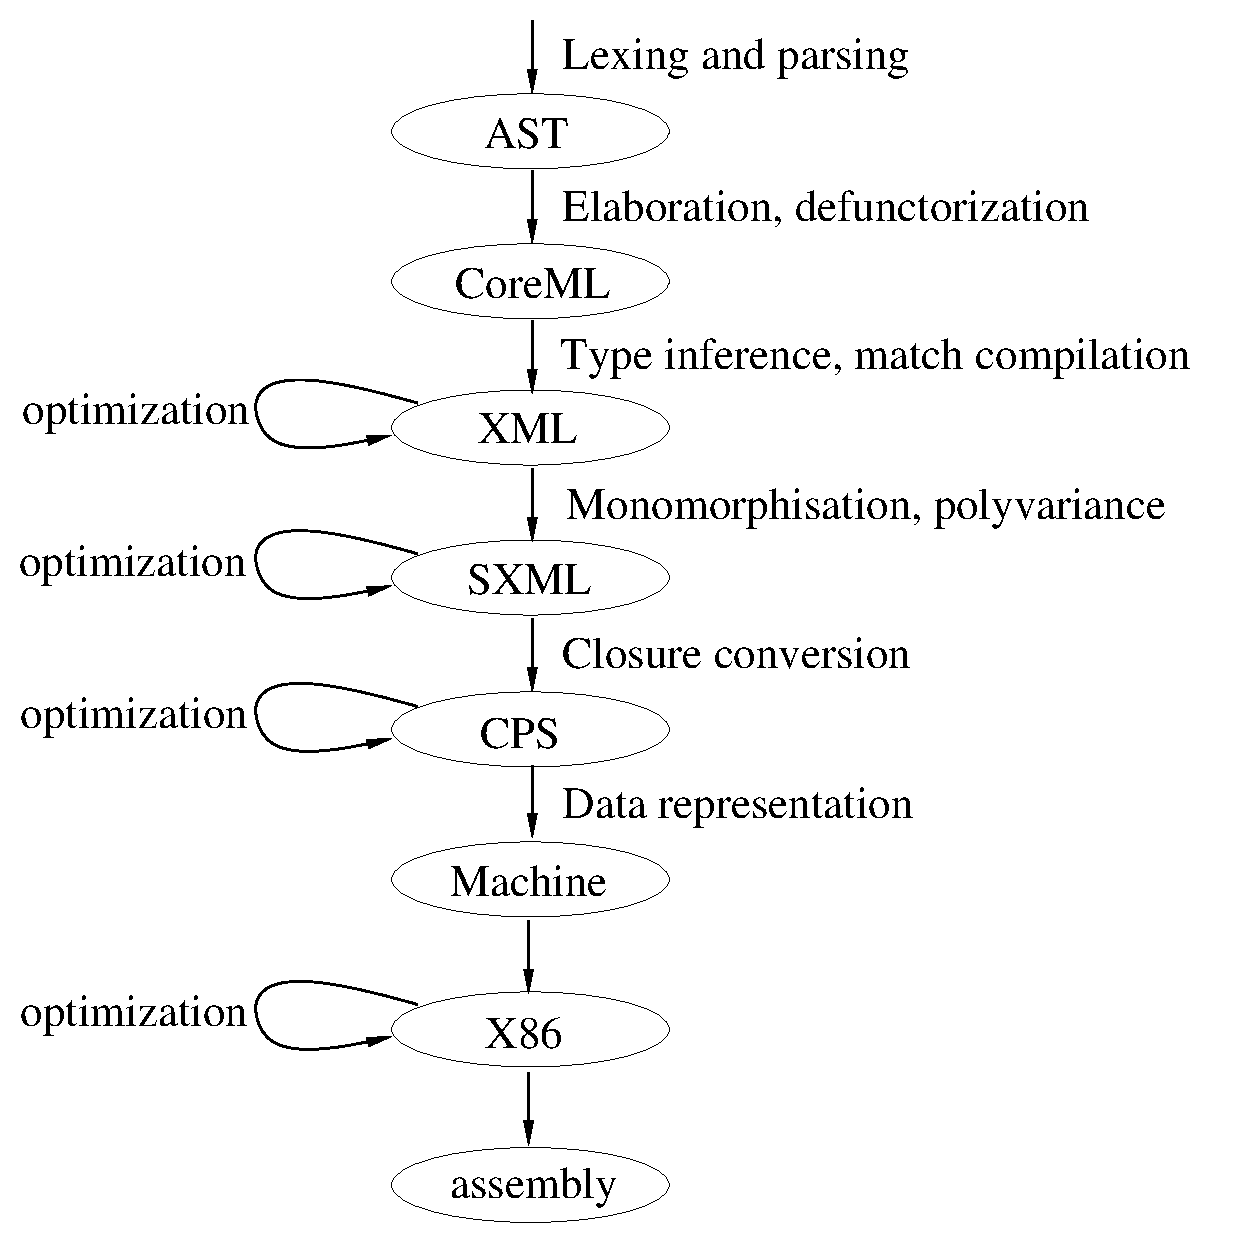
\epsfig{file=structure.eps,width=5.0in}}
\figEnd{Compiler structure}
       {structure}

The front end (\chapref{front-end}) takes SML source code (a complete
program) and performs lexing and parsing, producing an abstract syntax
tree (\chapref{ast}).  The lexer is produced by
ml-lex\cite{AppelEtAl94} and the parser is produced by
ml-yacc\cite{TarditiAppel94}.  The specifications for 
the lexer and parser were originally taken from \smlnj 109.32.  The
lexer is unchanged.  I have substantially modified the actions in the
grammar to produce my own version of abstract syntax trees (similar
to, but different from {\smlnj}).

Defunctorization (\chapref{defunctorization}), translates abstract
syntax trees to a small implicitly typed core language, called Core ML
(\chapref{core-ml}).  Its primary task is to eliminate all uses of the
module system (signatures, structures, functors).  It does this by
applying all functors and flattening all structures, moving
declarations to the top level.  This phase also performs precedence
parsing of infix expressions and patterns (the code to do this was
taken from \smlnj).  Finally, it does some amount of "macro
expansion", so that the core language is smaller.

Type inference (\chapref{type-inference}) translates implicitly typed
Core ML to an explicitly typed core language, XML (\chapref{xml}),
with explicit type abstraction and application.  XML is based on the
language ``Core-XML'' described in \cite{HarperMitchell93}.  Type
inference consists of two passes.  The first pass determines the
binding sites of type variables that are not explicitly bound (section
4.6 of the Definition).  The second pass is a
pretty standard unification based Hindley-Milner type
inference\cite{DamasMilner82}.  The type inference pass also performs
overloading resolution and resolution of flexible record patterns.
This pass also performs match compilation, by which I mean the
translation of case statements with nested patterns to (nested) case
statements with flat patterns.

Monomorphisation (\chapref{monomorphisation}) translates XML to its
simply-typed subset, called SXML (\chapref{sxml}), by duplicating all
polymorphic functions and datatypes for each type at which they are
instantiated.  Monomorphisation is only possible because SML has
``let-style'' polymorphism, in which all uses of a polymorphic value
are syntactically apparent (after functors are eliminated).

\chap{Notes}{notes}

This chapter contains random notes (usually old emails) on various
subtle issues.

\section{IntInf and Flattener}

\begin{verbatim}
From: "Stephen T. Weeks" <sweeks@intertrust.com>
Date: Tue, 27 Jun 2000 18:52:19 -0700 (PDT)
To: MLton@research.nj.nec.com
Subject: safe for space ... and IntInf
\end{verbatim}

Your mail also came at a fortunate time, as I was trying to track down
a seg fault I was getting in the smith-normal-form regression test.
For stress testing, I turned off all the cps simplify passes (except
for poly equal) and ran the regressions.  smith-normal-form failed
with a seg fault when compiled normally, and failed with an assertion
failure in \verb+IntInf_do_neg+ when compiled -g.  The assertion
failure was right at the beginning, checking that the frontier is in
the expected place.
\begin{verbatim}
         assert(frontier == (pointer)&bp->limbs[bp->card - 1]);
\end{verbatim}
I'd been tracking this bug for a couple hours when I received your
mail about the flattener.  Do you see the connection? :-)  As a
reminder, here is the code for \verb+bigNegate+
\begin{verbatim}
         fun bigNegate (arg: bigInt): bigInt =
                if Prim.isSmall arg
                      then let val argw = Prim.toWord arg
                           in if argw = badw
                                 then negBad
                                 else Prim.fromWord (Word.- (0w2, argw))
                           end
                      else Prim.~ (arg, allocate (1 + bigSize arg))
\end{verbatim}
The problem is, when the flattener is turned off, there is an
allocation in between the call to allocate and the \verb+Prim.~+ call.  The
argument tuple allocation screws everything up.  So, we are relying on 
the flattener for correctness of the IntInf implementation.  Any ideas 
on how to improve the implementation to remove this reliance, or at
least put an assert somewhere to avoid falling prey to this bug again?


\chap{Todo}{todo}
native backend vs x86 backend
To unpackage debian, do
\begin{verbatim}
dpkg -x ../mlton_20010806-2_i386.deb .
\end{verbatim}
\printindex
\bibliographystyle{alpha}
\bibliography{reference}
\end{document}
